\documentclass{article}
\usepackage{arxiv}

\usepackage[utf8]{inputenc} % allow utf-8 input
\usepackage[T1]{fontenc}    % use 8-bit T1 fonts
\usepackage{hyperref}       % hyperlinks
\usepackage{url}            % simple URL typesetting
\usepackage{booktabs}       % professional-quality tables
\usepackage{amsfonts,amssymb,amsmath}       % blackboard math symbols
\usepackage{nicefrac}       % compact symbols for 1/2, etc.
\usepackage{microtype}      % microtypography
\usepackage{lipsum}
\usepackage{graphicx}
\graphicspath{ {./images/} }


\title{Crypto Momentum Portfolios}


\author{
 Jules Prieux \\
  Paris-Dauphine University\\
  Paris, 75016  \\
  \texttt{jules.prieux@dauphine.eu} \\
  %% examples of more authors
   \And
 Ahmed Bachir \\
  Paris-Dauphine University\\
  Paris, 75016 \\
  \texttt{ahmed.bachir@dauphine.eu} \\
  \And
 Baptiste Zloch \\
  Paris-Dauphine University\\
  Paris, 75016 \\
  \texttt{baptiste.zloch@dauphine.eu} \\
  %% \AND
  %% Coauthor \\
  %% Affiliation \\
  %% Address \\
  %% \texttt{email} \\
  %% \And
  %% Coauthor \\
  %% Affiliation \\
  %% Address \\
  %% \texttt{email} \\
  %% \And
  %% Coauthor \\
  %% Affiliation \\
  %% Address \\
  %% \texttt{email} \\
}

\begin{document}
\maketitle
\begin{abstract}

	In the ever-evolving landscape of cryptocurrency investment, this research paper draws inspiration from financial luminaries Moskowitz et al. (2012) and \cite{buyingwinnerssellinglosers} to craft a sophisticated approach tailored to the unique characteristics of Bitcoin (BTC). \newline
	Our study undertakes a comprehensive exploration of the dataset's statistical properties and crafts bespoke momentum signals for cryptocurrency markets. Leveraging these signals, we design a cutting-edge quantitative investment strategy encompassing market timing for both long and short positions, along with long-short and long-only frameworks using a cross-sectional approach. We meticulously analyze historical price data to extract meaningful insights into the statistical nuances of the cryptocurrency market, fashioning robust momentum signals that align with the idiosyncrasies of digital assets. Our strategies empower active market participation, enabling investors to seize short-term trends in BTC performance. Through rigorous backtesting, we evaluate and compare strategy performance against a market cap-weighted benchmark.This research not only advances cryptocurrency investment strategies but also contributes to the broader discourse on applying traditional financial models to digital assets. By distilling our findings, we offer nuanced perspectives for academics and practitioners navigating the dynamic world of cryptocurrency investments.
\end{abstract}



\keywords{Cryptocurrencies \and Asset pricing \and Time series \and Portfolio management}
\section{Introduction}
\section{Data}
Jules
\section{Methodology}
\subsection{Notations}
In the following pages we present the methodology to run a momentum strategy against a benchmark. We use different notations
\begin{itemize}
	\item $X$ is the distribution of the return it could be parametric or non-parametric
	\item $r_{p_i}$ is the scalar representing the i-th daily return.
	\item $r_p$ is a vector representing all the returns of the portfolio
	\item $r_b$ is a vector representing all the returns of the benchmark
	\item $r_F$ is the scalar representing the risk-free rate
\end{itemize}

\subsection{Benchmarks definition}
We aim to conduct multiple backtests to assess the viability of momentum factor investing in cryptocurrencies. To evaluate the performance of the momentum strategy, it is imperative to establish baseline benchmarks. Accordingly, we will delineate three distinct benchmarks:
\begin{itemize}
	\item \textbf{A market capitalization weighted benchmark}: This benchmark encompasses the entire spectrum of cryptocurrencies, with weights allocated proportionally to the market capitalization of each asset.
	\item \textbf{An equally weighted benchmark}: This benchmark includes the entire array of cryptocurrencies, with each asset assigned an identical weight.
	\item \textbf{BTC-USDT benchmark}: Here, Bitcoin is employed as the benchmark due to its widespread recognition and status as the most extensively traded cryptocurrency.
\end{itemize}

\begin{figure} % picture
	\centering
	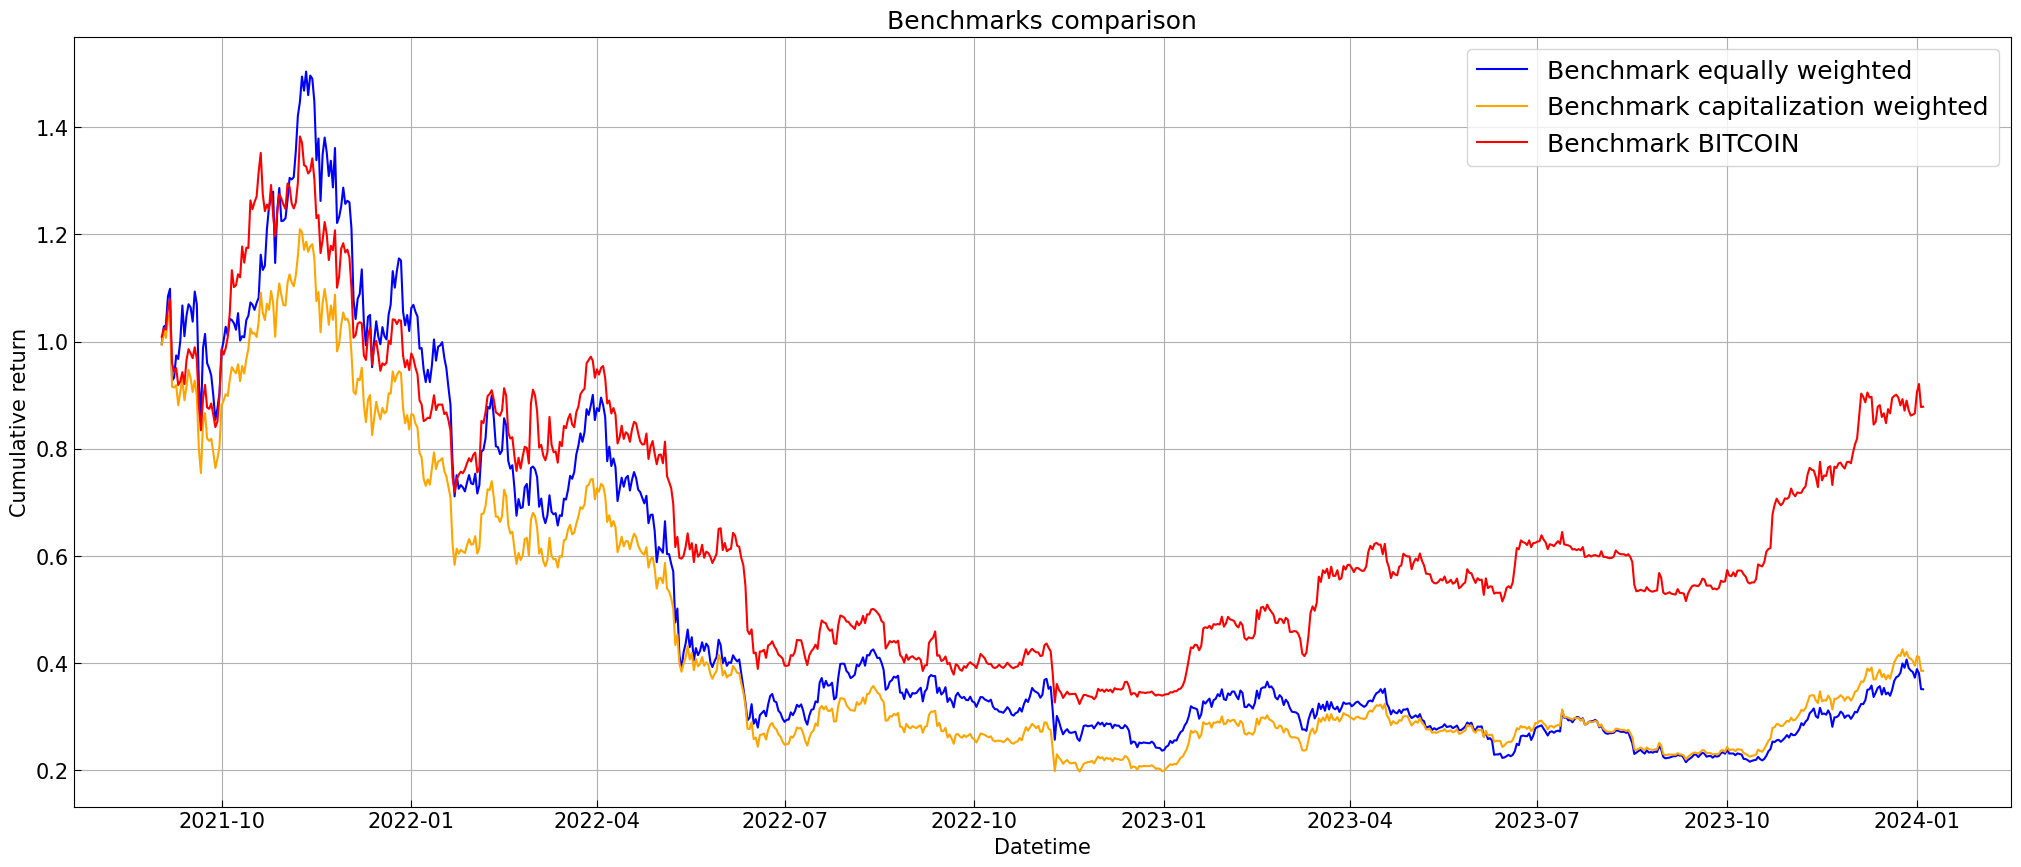
\includegraphics[width=1\linewidth]{benchmarks_only.png}
	\caption{The historical track of the 3 benchmarks used in this paper}
	\label{fig:fig1}
\end{figure}

\subsection{Performance and risk metrics}
To gauge the effectiveness of various iterations of the momentum strategy, we will employ the following set of performance metrics and risk metrics. All the metrics computed will be presented as annualized in the main result section.

The expected return is a scalar representing the gain or loss an investor can expected on average. $$r_P=\mathbb{E}[r_p]=\Bar{r_p}=\frac{1}{N}\sum_{i=1}^Nr_{p_i}$$
The historical volatility is a risk measure it is calculated the standard deviation of the returns around the mean over a certain period. $$\sigma_P = \sqrt{\frac{1}{N-1}\times\sum^N_{i=1}(r_{p_i}-\Bar{r_p})^2}$$
The historical value-at-risk (VaR) is a risk measure, it represents a percentile of the returns distribution usually it is a loss that could occur at $\alpha$ percent of the time. $$\text{VaR}_{1-\alpha}(X)=\text{inf}_{t\in\mathbb{R}}\{t:P(X\leq t)\geq1-\alpha\}$$
The historical conditional value-at-risk CVaR is the average loss for the extreme returns usually conditioned as lower than the value-at-risk. $$\text{CVaR}_{1-\alpha}(X)=\frac{1}{\alpha}\int_\alpha^\beta\text{VaR}_{1-\gamma}(X)d\gamma$$
Beta : $$\beta = \frac{\text{cov}(r_p,r_b)}{\sigma_B^2}$$
Tracking error : $$\text{TE}=\sqrt{\mathbb{V}(r_p-r_b)}$$
Sharpe ratio : $$\text{SR} = \frac{r_P-r_F}{\sigma_P}$$
Information ratio :$$\text{IR} = \frac{r_P-r_B}{TE}$$
Tail ratio : $$\text{TR}=\frac{\text{CVaR}_{0.05}(X)}{\text{CVaR}_{0.95}(X)}$$\newline


\subsection{Different momentum formula}
\subsection{Backtest implementation}
\subsection{Asset selection}
\subsection{Asset allocation}
\section{Descriptive statistics}
Ahmed
\section{Main results}
\subsection{Optimal momentum and rebalance period}
Jules
\subsection{Optimal momentum allocation}
Ahmed
\section{Robustness}

\section{Conclusion}
\section{References}
\section{Appendix}
\textbf{TEMPLATE EXAMPLE BELOW}
%%%%%%%%%%%%%%%%%%%%%%%%%%%%% TEMPLATE EXAMPLE BELOW %%%%%%%%%%%%%%%%%%%%%%%%%%%%%%%%%%%%%
\section{Introduction}
Our project is a competition on Kaggle (Predict Future Sales). We are provided with daily historical sales data (including each products’ sale date, block ,shop price and amount). And we will use it to forecast the total amount of each product sold next month. Because of the list of shops and products slightly changes every month. We need to create a robust model that can handle such situations.


\section{Task description and data construction}
\label{sec:headings}
We are provided with five datasets from Kaggle: Sales train, Sale test, items, item categories and shops. In the Sales train dataset, it provides the information about the sales’ number of an item in a shop within a day. In the Sales test dataset, it provides the shop id and item id which are the items and shops we need to predict. In the other three datasets, we can get the information about item’s name and its category, and the shops’ name.
\paragraph{Task modeling.}
We approach this task as a regression problem. For every item and shop pair, we need to predict its next month sales(a number).
\paragraph{Construct train and test data.}
In the Sales train dataset, it only provides the sale within one day, but we need to predict the sale of next month. So we sum the day's sale into month's sale group by item, shop, date(within a month).
In the Sales train dataset, it only contains two columns(item id and shop id). Because we need to provide the sales of next month, we add a date column for it, which stand for the date information of next month.

\subsection{Headings: second level}
\lipsum[5]
\begin{equation}
	\xi _{ij}(t)=P(x_{t}=i,x_{t+1}=j|y,v,w;\theta)= {\frac {\alpha _{i}(t)a^{w_t}_{ij}\beta _{j}(t+1)b^{v_{t+1}}_{j}(y_{t+1})}{\sum _{i=1}^{N} \sum _{j=1}^{N} \alpha _{i}(t)a^{w_t}_{ij}\beta _{j}(t+1)b^{v_{t+1}}_{j}(y_{t+1})}}
\end{equation}

\subsubsection{Headings: third level}
\lipsum[6]

\paragraph{Paragraph}
\lipsum[7]

\section{Examples of citations, figures, tables, references}
\label{sec:others}
\lipsum[8] \cite{kour2014real,kour2014fast} and see \cite{hadash2018estimate}.

The documentation for \verb+natbib+ may be found at
\begin{center}
	\url{http://mirrors.ctan.org/macros/latex/contrib/natbib/natnotes.pdf}
\end{center}
Of note is the command \verb+\citet+, which produces citations
appropriate for use in inline text.  For example,
\begin{verbatim}
   \citet{hasselmo} investigated\dots
\end{verbatim}
produces
\begin{quote}
	Hasselmo, et al.\ (1995) investigated\dots
\end{quote}

\begin{center}
	\url{https://www.ctan.org/pkg/booktabs}
\end{center}


\subsection{Figures}
\lipsum[10]
See Figure \ref{fig:fig1}. Here is how you add footnotes. \footnote{Sample of the first footnote.}
\lipsum[11]

\begin{figure}
	\centering
	\fbox{\rule[-.5cm]{4cm}{4cm} \rule[-.5cm]{4cm}{0cm}}
	\caption{Sample figure caption.}
	\label{fig:fig1}
\end{figure}

\begin{figure} % picture
	\centering
	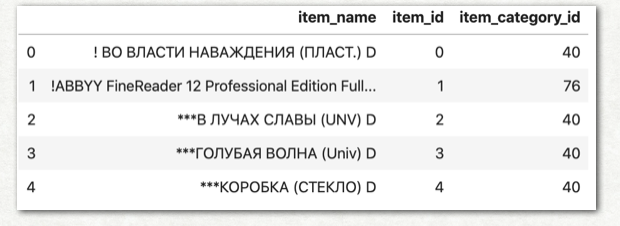
\includegraphics{test.png}
\end{figure}

\subsection{Tables}
\lipsum[12]
See awesome Table~\ref{tab:table}.

\begin{table}
	\caption{Sample table title}
	\centering
	\begin{tabular}{lll}
		\toprule
		\multicolumn{2}{c}{Part}                   \\
		\cmidrule(r){1-2}
		Name     & Description     & Size ($\mu$m) \\
		\midrule
		Dendrite & Input terminal  & $\sim$100     \\
		Axon     & Output terminal & $\sim$10      \\
		Soma     & Cell body       & up to $10^6$  \\
		\bottomrule
	\end{tabular}
	\label{tab:table}
\end{table}

\subsection{Lists}
\begin{itemize}
	\item Lorem ipsum dolor sit amet
	\item consectetur adipiscing elit.
	\item Aliquam dignissim blandit est, in dictum tortor gravida eget. In ac rutrum magna.
\end{itemize}


\bibliographystyle{unsrt}
%\bibliography{references}  %%% Remove comment to use the external .bib file (using bibtex).
%%% and comment out the ``thebibliography'' section.


%%% Comment out this section when you \bibliography{references} is enabled.
\begin{thebibliography}{1}

	\bibitem{kour2014real}
	George Kour and Raid Saabne.
	\newblock Real-time segmentation of on-line handwritten arabic script.
	\newblock In {\em Frontiers in Handwriting Recognition (ICFHR), 2014 14th
			International Conference on}, pages 417--422. IEEE, 2014.

	\bibitem{kour2014fast}
	George Kour and Raid Saabne.
	\newblock Fast classification of handwritten on-line arabic characters.
	\newblock In {\em Soft Computing and Pattern Recognition (SoCPaR), 2014 6th
			International Conference of}, pages 312--318. IEEE, 2014.

	\bibitem{hadash2018estimate}
	Guy Hadash, Einat Kermany, Boaz Carmeli, Ofer Lavi, George Kour, and Alon
	Jacovi.
	\newblock Estimate and replace: A novel approach to integrating deep neural
	networks with existing applications.
	\newblock {\em arXiv preprint arXiv:1804.09028}, 2018.

\end{thebibliography}


\end{document}
